\documentclass[]{scrartcl}
\usepackage{listings}
\usepackage{graphicx}

%opening
\title{Exercise Sheet 4: Intel Cilk and OpenCL}
\author{Gaurav Kukreja, Evangelos Drossos}

\begin{document}
\lstset{language=C}

\maketitle

\begin{abstract}

\end{abstract}

\section{Exercise 11}

\subsection{Advantages of Cilk and keywords needed}
Cilk is designed keeping in mind, that the developers and software producers
are not interested in rewriting the code, to exploit the benefits of parallelism.
Therefore it is designed in a way such that developers can exploit parallelism, by 
making small modifications to existing code. The resulting code continues to
perform on older machines with single processors, and makes us of parallel hardware
whenever possible.

Using Cilk is easier compared to other parallel programming constructs and frameworks.
It supports 3 keywords \textit{\_cilk\_spawn}, \textit{\_cilk\_sync} and \textit{\_cilk\_for}.

\subsubsection{cilk\_spawn}
This keywords modifies a function call statement to tell the runtime system that
the function may(but is not required to) run in parallel with the caller. This keyword
may be used as follows

\begin{lstlisting}
type var = cilk_spawn (func args) ; // func () returns a value
var = cilk_spawn func(args) ; // func () returns a value
cilk_spawn func(args) ; // func() may return void
\end{lstlisting}

\subsubsection{cilk\_sync}
The cilk\_sync statement indicates that the current function cannot continue in parallel with its
spawned children. After the children all complete, the current function can continue.

\begin{lstlisting}
cilk_sync;
\end{lstlisting}

This statement only syncs with children spawned by this function. Children of other functions are not affected.

\subsubsection{cilk\_for}
A cilk\_for loop is a replacement for the normal C/C++ for loop that permits loop iterations 
to run in parallel. The syntax is as follows

\begin{lstlisting}
cilk_for(declaration; 
		conditional expression; 
		increment expression)
body
\end{lstlisting}

There are some restrictions to use of cilk\_for. The loop must be simple, with uniform
stride length. The control variable, or iteration counter must not be changed inside the 
loop, other than in the increment expression of the cilk\_for statement. The termination
condition should be simple, and should not change between iterations.

\pagebreak
\subsection{Array Expressions with Intel C language extensions}
C/C++ language extensions for array notations is an Intel-specific language extension 
that is part of Intel Cilk Plus feature supported by Intel Compiler. The extension provides
following major benefits:

\begin{enumerate}
	\item Allows use of array notations to program parallel operations
	\item Achieves predictable performance based on mapping parallel constructs to the underlying multi-threaded and SIMD hardware.
	\item Enables compiler parallelization and vectorization with less reliance on alias and dependence analysis.
\end{enumerate}

\subsubsection{Array Section Notation}
A new section operator is introduced. 

\begin{lstlisting}
section_operator ::= [<lower_bound> : <length> : <stride>]
\end{lstlisting}

Here, \textit{lower\_bound}, \textit{length} and \textit{stride} are integers. The statement
represents a set of integer values as follows

\begin{verbatim}
<lower_bound>, <lower_bound + stride>, <lower_bound + 2*stride>,
 ... , <lower_bound + (length-1)*stride>
\end{verbatim}

A section operator can occur in place of a subscript operator. That is, elements of an array
a[lb], a[lb+str], a[lb+2*str], ..., a[lb + (len-1)*str] can be represented as a[lb:len:str].
Further usage of the section operator is illustrated as follows:

\begin{lstlisting}
a[0:3][0:4]	// refers to 12 elements in the 2-dimensional
		array starting at row 0, column 0, and ending
		at row 2,column 3
b[0:2:3] 	// refers to elements 0 and 3 of 1 dimensional
		array b
b[:] 		// refers to the entire array b
\end{lstlisting}

\subsubsection{Types of expressions}

\begin{itemize}

\item \textbf{Operators} \\
	Most C/C++ operators are available for array sections. Following expressions can be used.
	
	\begin{lstlisting}
a[:] * b[:]	//element-wise multiplication
a[0:3][0:3] + b[1:4][1:4] // matrix addition
a[0:3][0:3] + b[0][1] // allowed. adds scalar b[0][1] to an
	array section.
	\end{lstlisting}

	Operations between sections of different size will fail.

\item \textbf{Assignment} \\
	Assignment operator applies in parallel to every element of the array section.
	
	\begin{lstlisting}
a[0:3] = b[0:3] + c;
a[:][:] = d[:]; // error, different rank
	\end{lstlisting}

\item \textbf{Gather and Scatter} \\
	When an array section occurs directly under a subscript expression, it designates a set of elements indexed by the values of the array section.
	
	\begin{lstlisting}
unsigned index[10] = {0,1,2,3,4,5,6,7,8,9};
float out[10], in[10] = {9,8,7,6,5,4,3,2,1,0};
out[0:5] = in[index[0:5]]; // gather
out[index[5:5]] = in[0:5]; //scatter
for(int i = 0; i < 5; i++){
	cerr << "out[" << i << "]" << out[i] << endl;
}
	\end{lstlisting}

	\item \textbf{Reduction Operations} \\
	There are some built in Reduction functions which use the section operator e.g. 
	\textit{\_\_sec\_reduce\_add (a[:])}, which adds the values passed as arrays, and
	returns result. Similarly, following reduction functions are built-in.
	\begin{itemize}
		\item \texttt{\_\_sec\_reduce\_mul (a[:]) // multiplies all values in array}
		\item \texttt{\_\_sec\_reduce\_all\_zero (a[:]) // checks if all values are 0}
		\item \texttt{\_\_sec\_reduce\_all\_nonzero (a[:]) // checks if all values are not 0}
		\item \texttt{\_\_sec\_reduce\_any\_nonzero (a[:]) // tests for a value that is not 0}
		\item \texttt{\_\_sec\_reduce\_min (a[:] // returns minimum value}
		\item \texttt{\_\_sec\_reduce\_max (a[:])// returns maximum value}
		\item \texttt{\_\_sec\_reduce\_min\_ind (a[:]) // returns index of min value}
		\item \texttt{\_\_sec\_reduce\_max\_ind (a[:]) // returns index of max value}		
	\end{itemize}
	
	\item \textbf{Shift Operations}
	Intel Cilk PLus supports shift and rotate operations on array sections. The function
	prototypes are as follows
	
	\begin{lstlisting}
b[:] = __sec_shift(a[:], signed shift_val, fill_val) // Generic Shift Function
b[:] = __sec_rotate(a[:], signed shift_val) // Generic Rotate Function
	\end{lstlisting}
	
	\item Function Maps
	Maps are implicitly defined on scalar functions. They take array sections, and run on
	each element in parallel, with no specific ordering. For example,
	
	\begin{lstlisting}
a[:] = sin(b[:]);
a[:] = pow(b[:], c);
a[:] = pow(c, b[:]);
	\end{lstlisting}
\end{itemize}
	
\pagebreak
\subsection{Memory Structure in OpenCL}
OpenCL is a framework for exploiting parallel hardware found in CPUs, GPGPUs and
other special hardware. Unlike CUDA, OpenCL is designed to be compatible with a vast
variety of hardware. Therefore, OpenCL assumes a uniform hardware architecture for
the sake of its execution and memory model. The appropriate features provided by the
hardware are mapped to this architecture by the run-time system.

The following figure shows the hardware architecture assumed by OpenCL.

\begin{figure}[hb]
	\centering
	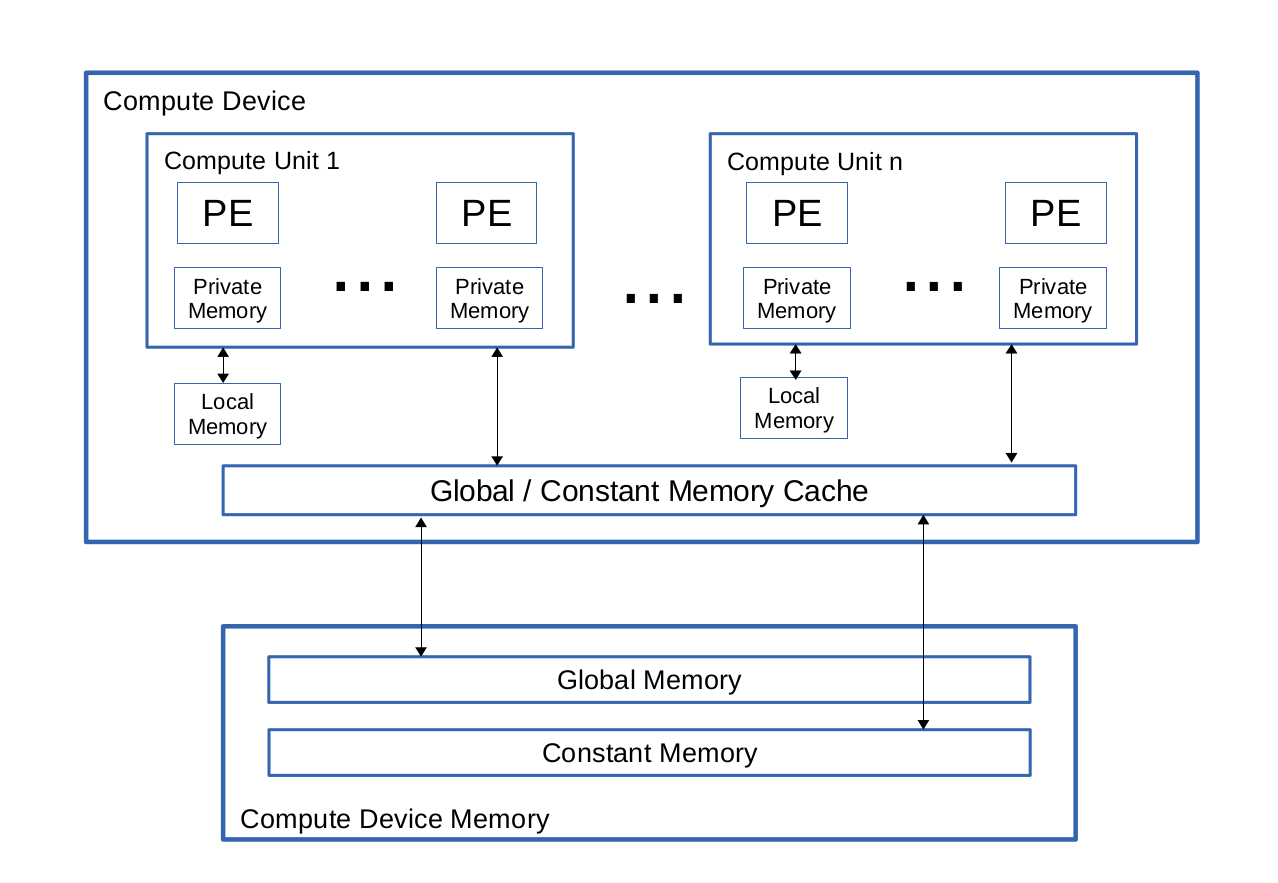
\includegraphics[width=0.8\textwidth]{opencl_memory}
	\caption{Memory and Hardware Structure in OpenCL}
\end{figure}

Let's consider GPGPUs for our reference Compute Device. The Compute Device consists of
several Compute Units (Arithmetic Logical Units that execute code). The Compute Device has
Global Memory, which can be accessed by all the compute units in the device. This is a high
latency memory. This memory can also be accessed by the Host Device (CPU). The host device
communicates with the Compute Device using this memory.

The Device also has a low latency Constant Memory. Like Global Memory, this memory can also
be accessed by all Compute Units, but none of the Compute Units can write to this memory. 
Only the Host (CPU) will write to this memory. This memory can be used to provide input data
which does not need to be modified during the execution of code. The actual hardware may not
have the Constant Memory, in which case the run-time system will simply use the Global Memory.

The device has a Global/Constant Memory Cache. The content of this memory cannot be directly
controlled by the Compute Units. This is low latency cache memory which is maintained by the
run-time system.

Local Memory is a low latency memory, which is private to each Compute Unit. One Compute Unit
may not access contents in another Units Local Memory. OpenCL provides programmers with the
facility to designate data that needs to be held in Local Memory. The actual hardware may not
have Local Memory, or may have only a small amount of Local Memory. In this case, the data will
be stored in Global Memory. 

For best results, the user must customize the code such that optimal use of the hardware
resources can be achieved.

\pagebreak
\subsection{OpenCL Execution Model and Compilation of OpenCL Application}
An OpenCL application consists of 2 parts
\begin{itemize}
	\item Device Code
	\item Host Code
\end{itemize}
Host code runs on the Host Device eg. CPU. The host code is compiled by a standard C
compiler like GCC. The host code contains boiler plate code, which is used to detect the
hardware available on the system, and check the features. The host code initializes the
hardware to be used. It then creates the executable device code. As per the application
demands, the kernel along with input data is transferred to the Compute Device and execution
is started. The Host then reads the result from the Compute Device.

The Device Code is written in a language very similar to C, but with some extra features
and some restrictions. Special hardware specific compilers are used to compile the Device Code.
The compiled Device code is called the kernel. The host code detects hardware(GPGPUs) on the 
system and selects an appropriate hardware. It then tries to find the corresponding compiler,
and compiles the Device Code to create the kernel.


\end{document}